\setbeamertemplate{caption}{\raggedright\insertcaption\par}
\begin{frame}[fragile]
\frametitle{the spectral sequence of a filtration}
Replace picture of space $X$ with $H_*(X)$
\begin{figure}
\begin{tikzcd}[row sep = tiny]
 t^0 & t^1 & t^2 & t^3  \\
\begin{tikzpicture}
\raggedright
 \tikzstyle{point}=[circle,thick,draw=black,fill=black,inner sep=0pt,minimum width=4pt,minimum height=4pt]
    \node (a)[point] at (0,0) {};
     \draw[color=white] (0,0) circle(1cm);
\end{tikzpicture} 
\arrow{r}{$t$} 
&
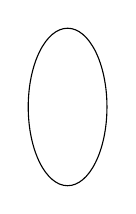
\begin{tikzpicture}
 \draw (0,0) arc (0:360:0.5cm and 1cm);
\end{tikzpicture} 
 \arrow{r}{$t$} 
&
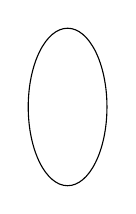
\begin{tikzpicture}
 \draw (0,0) arc (0:360:0.5cm and 1cm);
\end{tikzpicture} 
 \arrow{r}{$t$} 
&
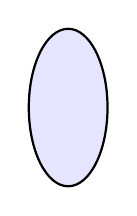
\begin{tikzpicture}
 \draw[thick,fill=blue!20!white,fill opacity=0.50] (0,0) arc (0:360:0.5cm and 1cm);
\end{tikzpicture}
\end{tikzcd}
\caption{{\color{blue}{Page 0:}} Input}
\end{figure}
\end{frame}

%%% PAGE 1

\setbeamertemplate{caption}{\raggedright\insertcaption\par}

\begin{frame}[fragile]
\frametitle{the spectral sequence of a filtration}
Replace picture of space $X$ with $H_*(X)$
\begin{figure}
\centering
\begin{tikzcd}[row sep = large]

\begin{tikzpicture}
 \tikzstyle{point}=[circle,thick,draw=black,fill=black,inner sep=0pt,minimum width=4pt,minimum height=4pt]
    \node (a)[point] at (0,0) {};
    % \draw[color=white] (0,0) circle(1cm);
\end{tikzpicture} 
\arrow{r}{$t$} \arrow{d}{$j$} 
&
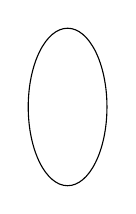
\begin{tikzpicture}
 \draw (0,0) arc (0:360:0.5cm and 1cm);
\end{tikzpicture}  
 \arrow{r}{$t$} \arrow{d}{$j$}
&
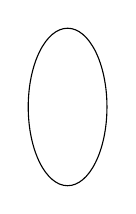
\begin{tikzpicture}
 \draw (0,0) arc (0:360:0.5cm and 1cm);
\end{tikzpicture}  
 \arrow{r}{$t$} \arrow{d}{$j$}
&
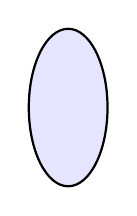
\begin{tikzpicture}
 \draw[thick,fill=blue!20!white,fill opacity=0.50] (0,0) arc (0:360:0.5cm and 1cm);
\end{tikzpicture}
\arrow{d}{$j$}
\\

\begin{tikzpicture}
 \tikzstyle{point}=[circle,thick,draw=black,fill=black,inner sep=0pt,minimum width=4pt,minimum height=4pt]
    \node (a)[point] at (0,0) {};
    % \draw[color=white] (0,0) circle(1cm);
\end{tikzpicture} 
&
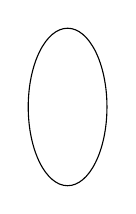
\begin{tikzpicture}
 \draw (0,0) arc (0:360:0.5cm and 1cm);
\end{tikzpicture}
\only<2->{\arrow{lu}{\delta}}
\only<3->{\arrow[dashed]{l}{d_1}} 
&

\begin{tikzpicture}
\tikzstyle{point}=[circle,thick,draw=black,fill=black,inner sep=0pt,minimum width=4pt,minimum height=4pt]
    \node (a)[point] at (0,0) {};
\end{tikzpicture}
\only<2->{\arrow{lu}{\delta}}
\only<3->{\arrow[dashed]{l}{d_1}} 
&
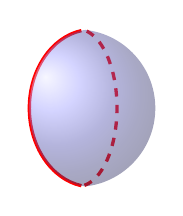
\begin{tikzpicture}
   \draw[very thick, dashed, red] (.1,-.98) arc (-80:85:.5cm and 1cm);
   \draw [very thick, red] (-.6,0) arc (180:100:.8cm and 1cm); 
    \draw [very thick, red] (-.6,0) arc (180:260:.8cm and 1cm); 
    \begin{scope}
     \clip (1,0) arc (0:360:0.8cm and 1cm);
    \shade[ball color=blue!50!white,opacity=0.45] (0,0) circle (1cm);
    \end{scope}
\end{tikzpicture}
\only<2->{\arrow{lu}{\delta}}
\only<3->{\arrow[dashed]{l}{d_1}}
\end{tikzcd}
\only<1>{\caption{{\color{blue}{Page 1:}} $H_*(X_t, X_{t-1})$}}
\only<2>{\caption{$\delta$: connecting homomorphism}}
\only<3>{\caption{{\color{blue}{Differentials: }}$d_1: j \circ \delta$}}
\end{figure}
\end{frame}

%% PAGE 2
\begin{frame}[fragile]
\frametitle{the spectral sequence of a filtration}
Replace picture of space $X$ with $H_*(X)$
\begin{figure}
\centering
\begin{tikzcd}[row sep = large]

\begin{tikzpicture}
 \tikzstyle{point}=[circle,thick,draw=black,fill=black,inner sep=0pt,minimum width=4pt,minimum height=4pt]
    \node (a)[point] at (0,0) {};
    % \draw[color=white] (0,0) circle(1cm);
\end{tikzpicture} 
\arrow{r}{$t$} \arrow{d}{$j$} 
&
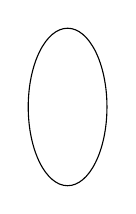
\begin{tikzpicture}
 \draw (0,0) arc (0:360:0.5cm and 1cm);
\end{tikzpicture}  
 \arrow{r}{$t$} \arrow{d}{$j$}
&
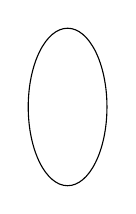
\begin{tikzpicture}
 \draw (0,0) arc (0:360:0.5cm and 1cm);
\end{tikzpicture}  
 \arrow{r}{$t$} \arrow{d}{$j$}
&
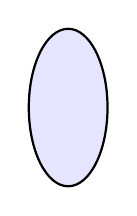
\begin{tikzpicture}
 \draw[thick,fill=blue!20!white,fill opacity=0.50] (0,0) arc (0:360:0.5cm and 1cm);
\end{tikzpicture}
\arrow{d}{$j$}
\\

\begin{tikzpicture}
 \tikzstyle{point}=[circle,thick,draw=black,fill=black,inner sep=0pt,minimum width=4pt,minimum height=4pt]
    \node (a)[point] at (0,0) {};
    % \draw[color=white] (0,0) circle(1cm);
\end{tikzpicture} 
&
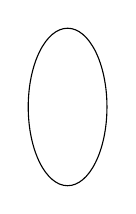
\begin{tikzpicture}
 \draw (0,0) arc (0:360:0.5cm and 1cm);
\end{tikzpicture}
\arrow{lu}{\delta}
\arrow[dashed]{l}{d_1}
&

\begin{tikzpicture}
\tikzstyle{point}=[circle,thick,draw=black,fill=black,inner sep=0pt,minimum width=4pt,minimum height=4pt]
    \node (a)[point] at (0,0) {};
\end{tikzpicture}
\arrow{lu}{\delta}
\arrow[dashed]{l}{d_1}
\only<2->{\arrow[dashed, bend left=90]{ll}{d_2}}
&
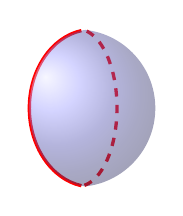
\begin{tikzpicture}
   \draw[very thick, dashed, red] (.1,-.98) arc (-80:85:.5cm and 1cm);
   \draw [very thick, red] (-.6,0) arc (180:100:.8cm and 1cm); 
    \draw [very thick, red] (-.6,0) arc (180:260:.8cm and 1cm); 
    \begin{scope}
     \clip (1,0) arc (0:360:0.8cm and 1cm);
    \shade[ball color=blue!50!white,opacity=0.45] (0,0) circle (1cm);
    \end{scope}
\end{tikzpicture}
\arrow{lu}{\delta}
\arrow[dashed]{l}{d_1}
\only<2->{\arrow[dashed, bend left=45]{ll}{d_2}}
\end{tikzcd}
\only<1>{\caption{{\color{blue}{Page 2:}} Compute Homology of $d_1$}}
\only<2>{\caption{$d_2: j \circ t^{-1} \circ \partial$}}
\end{figure}
\end{frame}

%% DONE
\begin{frame}[fragile]
\frametitle{spectral sequences for applied topologists}
\begin{minipage}{.4\textwidth}
\hspace*{-1cm}
\begin{tikzcd}[row sep = normal]

\begin{tikzpicture}[scale=.4]
 \tikzstyle{point}=[circle,thick,draw=black,fill=black,inner sep=0pt,minimum width=4pt,minimum height=4pt]
    \node (a)[point] at (0,0) {};
    % \draw[color=white] (0,0) circle(1cm);
\end{tikzpicture} 
\arrow{r}{$t$} \arrow{d}{$j$} 
&

\begin{tikzpicture}[scale=.4]
 \draw (0,0) arc (0:360:0.5cm and 1cm);
\end{tikzpicture}  
 \arrow{r}{$t$} \arrow{d}{$j$}
&

\begin{tikzpicture}[scale=.4]
 \draw (0,0) arc (0:360:0.5cm and 1cm);
\end{tikzpicture}  
 \arrow{r}{$t$} \arrow{d}{$j$}
&
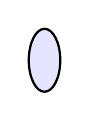
\begin{tikzpicture}[scale=.4]
 \draw[thick,fill=blue!20!white,fill opacity=0.50] (0,0) arc (0:360:0.5cm and 1cm);
\end{tikzpicture}
\arrow{d}{$j$}
\\

\begin{tikzpicture}[scale=.4]
 \tikzstyle{point}=[circle,thick,draw=black,fill=black,inner sep=0pt,minimum width=4pt,minimum height=4pt]
    \node (a)[point] at (0,0) {};
    % \draw[color=white] (0,0) circle(1cm);
\end{tikzpicture} 
&

\begin{tikzpicture}[scale=.4]
 \draw (0,0) arc (0:360:0.5cm and 1cm);
\end{tikzpicture}
\arrow{lu}{\delta}
\arrow[dashed]{l}{d_1}
&

\begin{tikzpicture}[scale=.4]
\tikzstyle{point}=[circle,thick,draw=black,fill=black,inner sep=0pt,minimum width=4pt,minimum height=4pt]
    \node (a)[point] at (0,0) {};
\end{tikzpicture}
\arrow{lu}{\delta}
\arrow[dashed]{l}{d_1}
\arrow[dashed, bend left=90]{ll}{d_2}
&
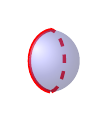
\begin{tikzpicture}[scale=.4]
   \draw[very thick, dashed, red] (.1,-.98) arc (-80:85:.5cm and 1cm);
   \draw [very thick, red] (-.6,0) arc (180:100:.8cm and 1cm); 
    \draw [very thick, red] (-.6,0) arc (180:260:.8cm and 1cm); 
    \begin{scope}
     \clip (1,0) arc (0:360:0.8cm and 1cm);
    \shade[ball color=blue!50!white,opacity=0.45] (0,0) circle (1cm);
    \end{scope}
\end{tikzpicture}
\arrow{lu}{\delta}
\arrow[dashed]{l}{d_1}
\arrow[dashed, bend left=45]{ll}{d_2}
\end{tikzcd}
\end{minipage}
\begin{minipage}{.5\textwidth}
\hspace*{4in}
\begin{itemize}
\item Page $n$ resolves persistence intervals of length $n$
\item<2-> Out of order execution $\Rightarrow$ less arithmetic.  (Bauer, Kerber, et. al)
\item<3-> \textbf{Issue: } No obvious control over memory usage.
\item<4-> \textbf{Morally: } Decomposes direct sum the wrong way
\item<5-> \textbf{Want: } Decompose many bars at once with less communication.
\item<6-> In other words, computation using a spatial division of the input 
\end{itemize}
\end{minipage}
\end{frame}
\setbeamertemplate{caption}[default]